\chapter{Appendices}
\label{appendices}

\section{Application Breakdown}
\label{sec:appbreakdnown}
The following section is a breakdown of the application into its various packages and files.
\subsection{Java Source}
\subsubsection{Package: beans}
\begin{table}[H]
\begin{center}
    \begin{tabular}{| l | l | l| l |p{1cm} |}
    \hline
    File Name & File Type & Function & No. Lines\\ \hline
    beans.xml & XML & Context Component Scan, Datasource Definition & 27 \\ \hline
	dao-context.xml & XML & DB Config, Database Exception Translator & 49 \\ \hline
	security-context.xml & XML & Security Configuration, Access Control & 118 \\ \hline
	service.xml & XML & Service Configuration & 10 \\ \hline
    \end{tabular}
\end{center}
\caption{beans package}
\end{table}

\subsubsection{Package: controllers}
\begin{table}[H]
\begin{center}
   \begin{tabular}{| l | l | l| l |p{1cm} |}
    \hline
    File Name & File Type & Function & No. Lines\\ \hline
    ErrorHandler & JAVA & Handles application errors & 30 \\ \hline
	EventController & JAVA & Handles Event actions & 108\\ \hline
	HomeControler & JAVA & Displays Home Page & 52\\ \hline
	JSONController & JAVA & Manages webservices & 78\\ \hline
	LoginController & JAVA & Manages user login & 23\\ \hline
	MembersController & JAVA & Handles Member actions &  582\\ \hline
	NewsController & JAVA & Handles display and creation of News  & 100\\ \hline
	RoleController & JAVA & Manages roles & 76 \\ \hline
	SiteController & JAVA & Displays site pages with static data & 52\\ \hline
	TimetableController & JAVA & Timetable Creation and Display & 708 \\ \hline
	TournamentController & JAVA & Management of Tournaments & 333 \\ \hline
    \end{tabular}
\end{center}
\caption{controllers package}
\end{table}

\subsubsection{Package: dao}
\begin{table}[H]
\begin{center}
    \begin{tabular}{| l | l | l| l |p{1cm} |}
    \hline
    File Name & File Type & Function & No. Lines\\ \hline
    EventDAO & JAVA & DAO for IEvent & 120 \\ \hline
	LogDAO & JAVA & DAO for ILog & 50\\ \hline
	NewsDAO & JAVA & DAO for News & 62\\ \hline
	RoleDAO & JAVA & DAO for Role & 110 \\ \hline
	TimetableDAO & JAVA & DAO for Timetable & 171\\ \hline
	TournamentDAO & JAVA & DAO for Tournament & 116\\ \hline
	UserDAO & JAVA & DAO for User & 318 \\ \hline
	UserRowMapper & JAVA & JDBC Row Mapper to handle multiple User objects & 30\\ \hline	
    \end{tabular}
\end{center}
\caption{dao package}
\end{table}

\subsubsection{Package: email}
\begin{table}[H]
\begin{center}
     \begin{tabular}{| l | l | l| l |p{1cm} |}
    \hline
    File Name & File Type & Function & No. Lines\\ \hline
    Email & JAVA & Create and Send Email Message & 70\\ \hline
	IEmail & JAVA & Interface for Email class & 12\\ \hline	
    \end{tabular}
\end{center}
\caption{email package}
\end{table}

\subsubsection{Package: events}
\begin{table}[H]
\begin{center}
      \begin{tabular}{| l | l | l| l |p{1cm} |}
    \hline
    File Name & File Type & Function & No. Lines\\ \hline
    Event & JAVA & Defines an event used by the Timetable & 74\\ \hline
	IEvent & JAVA & Interface for Event class & 5\\ \hline	
    \end{tabular}
\end{center}
\caption{event package}
\end{table}

\subsubsection{Package: events.tournaments}
\begin{table}[H]
\begin{center}
     \begin{tabular}{| l | l | l| l |p{1cm} |}
    \hline
    File Name & File Type & Function & No. Lines\\ \hline
    Tournament & JAVA & Defines an Tournament object & 140\\ \hline
	BasicTournamentSort & JAVA & Tournament Sort Implementation & 37\\ \hline
	ITournamentSorter & JAVA & Tournament Sort Interface & 10\\ \hline
    \end{tabular}
\end{center}
\caption{events.tournament package}
\end{table}

\subsubsection{Package: logs}
\begin{table}[H]
\begin{center}
    \begin{tabular}{| l | l | l| l |p{1cm} |}
    \hline
    File Name & File Type & Function & No. Lines\\ \hline
    Log & JAVA & Defines the structure of a system log file & 80\\ \hline
	ILog & JAVA & Interface for Log class & 2\\ \hline
    \end{tabular}
\end{center}
\caption{log package}
\end{table}

\subsubsection{Package: news}
\begin{table}[H]
\begin{center}
     \begin{tabular}{| l | l | l| l |p{1cm} |}
    \hline
    File Name & File Type & Function & No. Lines\\ \hline
    News & JAVA & Defines the structure of a News object & 55\\ \hline
    \end{tabular}
\end{center}
\caption{news package}
\end{table}

\subsubsection{Package: properties}
\begin{table}[H]
\begin{center}
     \begin{tabular}{| l | l | l| l |p{1cm} |}
    \hline
    File Name & File Type & Function & No. Lines\\ \hline
    jdbc & PROPERTIES & Holds log in values for the JDBC connection & 4\\ \hline
	mail & PROPERTIES & Holds the log in values for the email system & 2\\ \hline
    \end{tabular}
\end{center}
\caption{properties package}
\end{table}

\subsubsection{Package: reports}
\begin{table}[H]
\begin{center}
     \begin{tabular}{| l | l | l| l |p{1cm} |}
    \hline
    File Name & File Type & Function & No. Lines\\ \hline
    IReport & JAVA & Interface for Reports & 5\\ \hline
	CSVCreator & JAVA & Creates a CSV file for User Data & 122\\ \hline
    \end{tabular}
\end{center}
\caption{reports package}
\end{table}

\subsubsection{Package: service}
\begin{table}[H]
\begin{center}
      \begin{tabular}{| l | l | l| l |p{1cm} |}
    \hline
    File Name & File Type & Function & No. Lines\\ \hline
	EmailService & JAVA & Class for sending Emails & 49\\ \hline
    EventService & JAVA & Layer between Controller and DAO & 80\\ \hline
    LogService & JAVA & Layer between Controllers and DAO & 34\\ \hline
	NewsService & JAVA & Layer between Controller and DAO & 44\\ \hline
	RoleService & JAVA & Layer between Controllers and RoleDAO & 64\\ \hline
	TimetableService & JAVA & Layer between Controller and DAO & 80\\ \hline
	TournamentService & JAVA & Layer between Controller and DAO & 76\\ \hline
	UserService & JAVA & Layer between MemberController and UserDAO & 113\\ \hline
    \end{tabular}
\end{center}
\caption{service package}
\end{table}

\subsubsection{Package: timetable}
\begin{table}[H]
\begin{center}
    \begin{tabular}{| l | l | l| l |p{1cm} |}
    \hline
    File Name & File Type & Function & No. Lines\\ \hline
    Timetable & JAVA & Interface for Timetable & 48\\ \hline
	MonaleenTTV1 & JAVA & Defines structure and behaviour of Timetable object & 276\\ \hline
    \end{tabular}
\end{center}
\caption{timetable package}
\end{table}

\subsubsection{Package: users}
\begin{table}[H]
\begin{center}
    \begin{tabular}{| l | l | l| l |p{1cm} |}
    \hline
    File Name & File Type & Function & No. Lines\\ \hline
    FormValidationGroup & JAVA & Form Validation Class & n/a\\ \hline
	PersistenceValidationGroup & JAVA & Hibernate Validation Class & n/a\\ \hline
	Grade & JAVA & Defines structure of a Grade object& 40\\ \hline
	User & JAVA & Defines structure of a User object & 276\\ \hline
	Role & JAVA & Defines structure of Role object& 60\\ \hline	
    \end{tabular}
\end{center}
\caption{reports package}
\end{table}

\section{Apache Struts and JSP Pages}

\subsubsection{layout}
\begin{table}[H]
\begin{center}
   \begin{tabular}{| l | l | l| l |p{1cm} |}
    \hline
    File Name & File Type & Function & No. Lines\\ \hline
	default & XML & Defines the structure for each JSP page in the application & 269\\ \hline	
    \end{tabular}
\end{center}
\caption{struts layout}
\end{table}

\subsubsection{templates}
\begin{table}[H]
\begin{center}
\begin{tabular}{| l | l | l| l |p{1cm} |}
    \hline
    File Name & File Type & Function & No. Lines\\ \hline
	default & JSP & The JSP page used as a template& 39\\ \hline	
    \end{tabular}
\end{center}
\caption{templates layout}
\end{table}

\subsubsection{tiles}
\begin{table}[H]
\begin{center}
     \begin{tabular}{| l | l | l| l |p{1cm} |}
    \hline
    File Name & File Type & Function & No. Lines\\ \hline
	accessdenied & JSP & Access Denied page & 2\\ \hline
	adtennis & JSP & Alternate banner & 26\\ \hline	
	adtour & JSP & Alternate banner & 26\\ \hline	
	ad1 & JSP & Alternate banner & 26\\ \hline	
	adbanner & JSP & Alternate banner & 26\\ \hline		
	admin & JSP & Administrator page with admin options & 100\\ \hline	
	adminAnalysis & JSP & Displays site analytics & 165\\ \hline	
	adminEditProfile & JSP & Admin edit user accounts & 20\\ \hline	
	alreadyReg & JSP & Error for duplicate registration & 1 \\ \hline	
	approveMembers & JSP & Admin approve members page & 30\\ \hline	
	blockMembers & JSP & Admin suspend members page & 29\\ \hline	
	bookingExists & JSP & Error page to handle duplicate bookings & 1\\ \hline	
	checkRegistered & JSP & Displays users registered for a selected tournament & 12\\ \hline	
	chooseEdit & JSP & Choice for which Timetable to edit & 28\\ \hline	
	confirmEdit & JSP & Layout for editing individual slots in Timetable & 40\\ \hline	
	contactus & JSP & Contact Us page for application & 58\\ \hline	
	content & JSP & Place-holder page for default JSP template & 1\\ \hline	
	court & JSP & Displays selected Timetable and available options & 527\\ \hline	
	createEvent & JSP & Admin Create Event page & 8\\ \hline	
	createmembers & JSP & User Registration page & 152\\ \hline	
	createNewRole & JSP & Admin create new User Role & 31\\ \hline	
	createNews & JSP & Admin Create News page & 28\\ \hline	
	createTimetable & JSP & Admin Create Timetable page & 22\\ \hline	
	createTournament & JSP & Admin Create Tournament page & 13\\ \hline	
	deleteNews & JSP & Admin Delete News entry & 26\\ \hline	
	deleteTimetable & JSP & Admin Delete Timetable object & 30\\ \hline	
	deleteTournament & JSP & Admin Delete Tournament object & 37\\ \hline	
	displayUsers & JSP & Admin Displays all users to choose which one to edit & 24\\ \hline	
	editDetails & JSP & User Edit Profile & 74\\ \hline	
	emailAllMembers & JSP & Send message to all approved members & 11\\ \hline	
	emailSent & JSP & Email Sent Confirmation Page & 1\\ \hline	
	error & JSP & Default Error Page. Displays Class Error & 2\\ \hline	
	fillTimetable & JSP & Create Timetable template for series & 46\\ \hline	
    \end{tabular}
\end{center}
\end{table}
\pagebreak

\begin{table}[H]
\begin{center}
    \begin{tabular}{| l | l | l| l |p{1cm} |}
    \hline
    File Name & File Type & Function & No. Lines\\ \hline
	index & JSP & Default Home page & 96\\ \hline
	footer & JSP & Place-holder page for default JSP template & 1\\ \hline	
	header & JSP & Place-holder page for default JSP template & 62\\ \hline		
	links & JSP & Displays Site Navigation links & 26\\ \hline	
	loggedout & JSP & Logout Confirmation page & 1\\ \hline	
	login & JSP & Login Page - Linked to Spring Security & 32\\ \hline	
	maps & JSP & Displays Google Maps Location for Club & 28\\ \hline	
	members & JSP & Members Address Book for authenticated users & 22\\ \hline	
	membership & JSP & Displays Membership Information & 24\\ \hline	
	mobile & JSP & Displays JSON service & 14\\ \hline
	news & JSP & Displays News Page & 16\\ \hline	
	profile & JSP & Displays User Profile & 15\\ \hline	
	profileUpdated & JSP & Confirmation of profile being updated & 1\\ \hline	
	registerSuccess & JSP & Confirmation that user has successfully registered & 2\\ \hline	
	resetAllTimetable & JSP & Removes all bookings for a Timetable & 21\\ \hline	
	seriesChoice & JSP & Choose which Timetable series to edit/reset & 22\\ \hline	
	sortPreview & JSP & Preview of Tournament Sort & 14\\ \hline	
	timetable & JSP & Displays enabled timetables for users & 21 \\ \hline	
	timetableStatus & JSP & Allows admin to enable or disable timetables & 29\\ \hline	
	tournaments & JSP & Displays Enabled Tournaments for Users & 85\\ \hline	
	tournamentStatus & JSP & Admin to modify tournaments & 146\\ \hline	
	tournamentSuccess & JSP & Successful tournament creation & 1\\ \hline	
	training & JSP & Club training information & 2\\ \hline
	viewAllMembers & JSP & Admin View of Members & 67\\ \hline	
	viewEvents & JSP & Admin Event Management & 55\\ \hline	
    \end{tabular}
\end{center}
\caption{templates layout}
\end{table}

\section{Permission Letter}

\begin{figure}[H]
\begin{center}
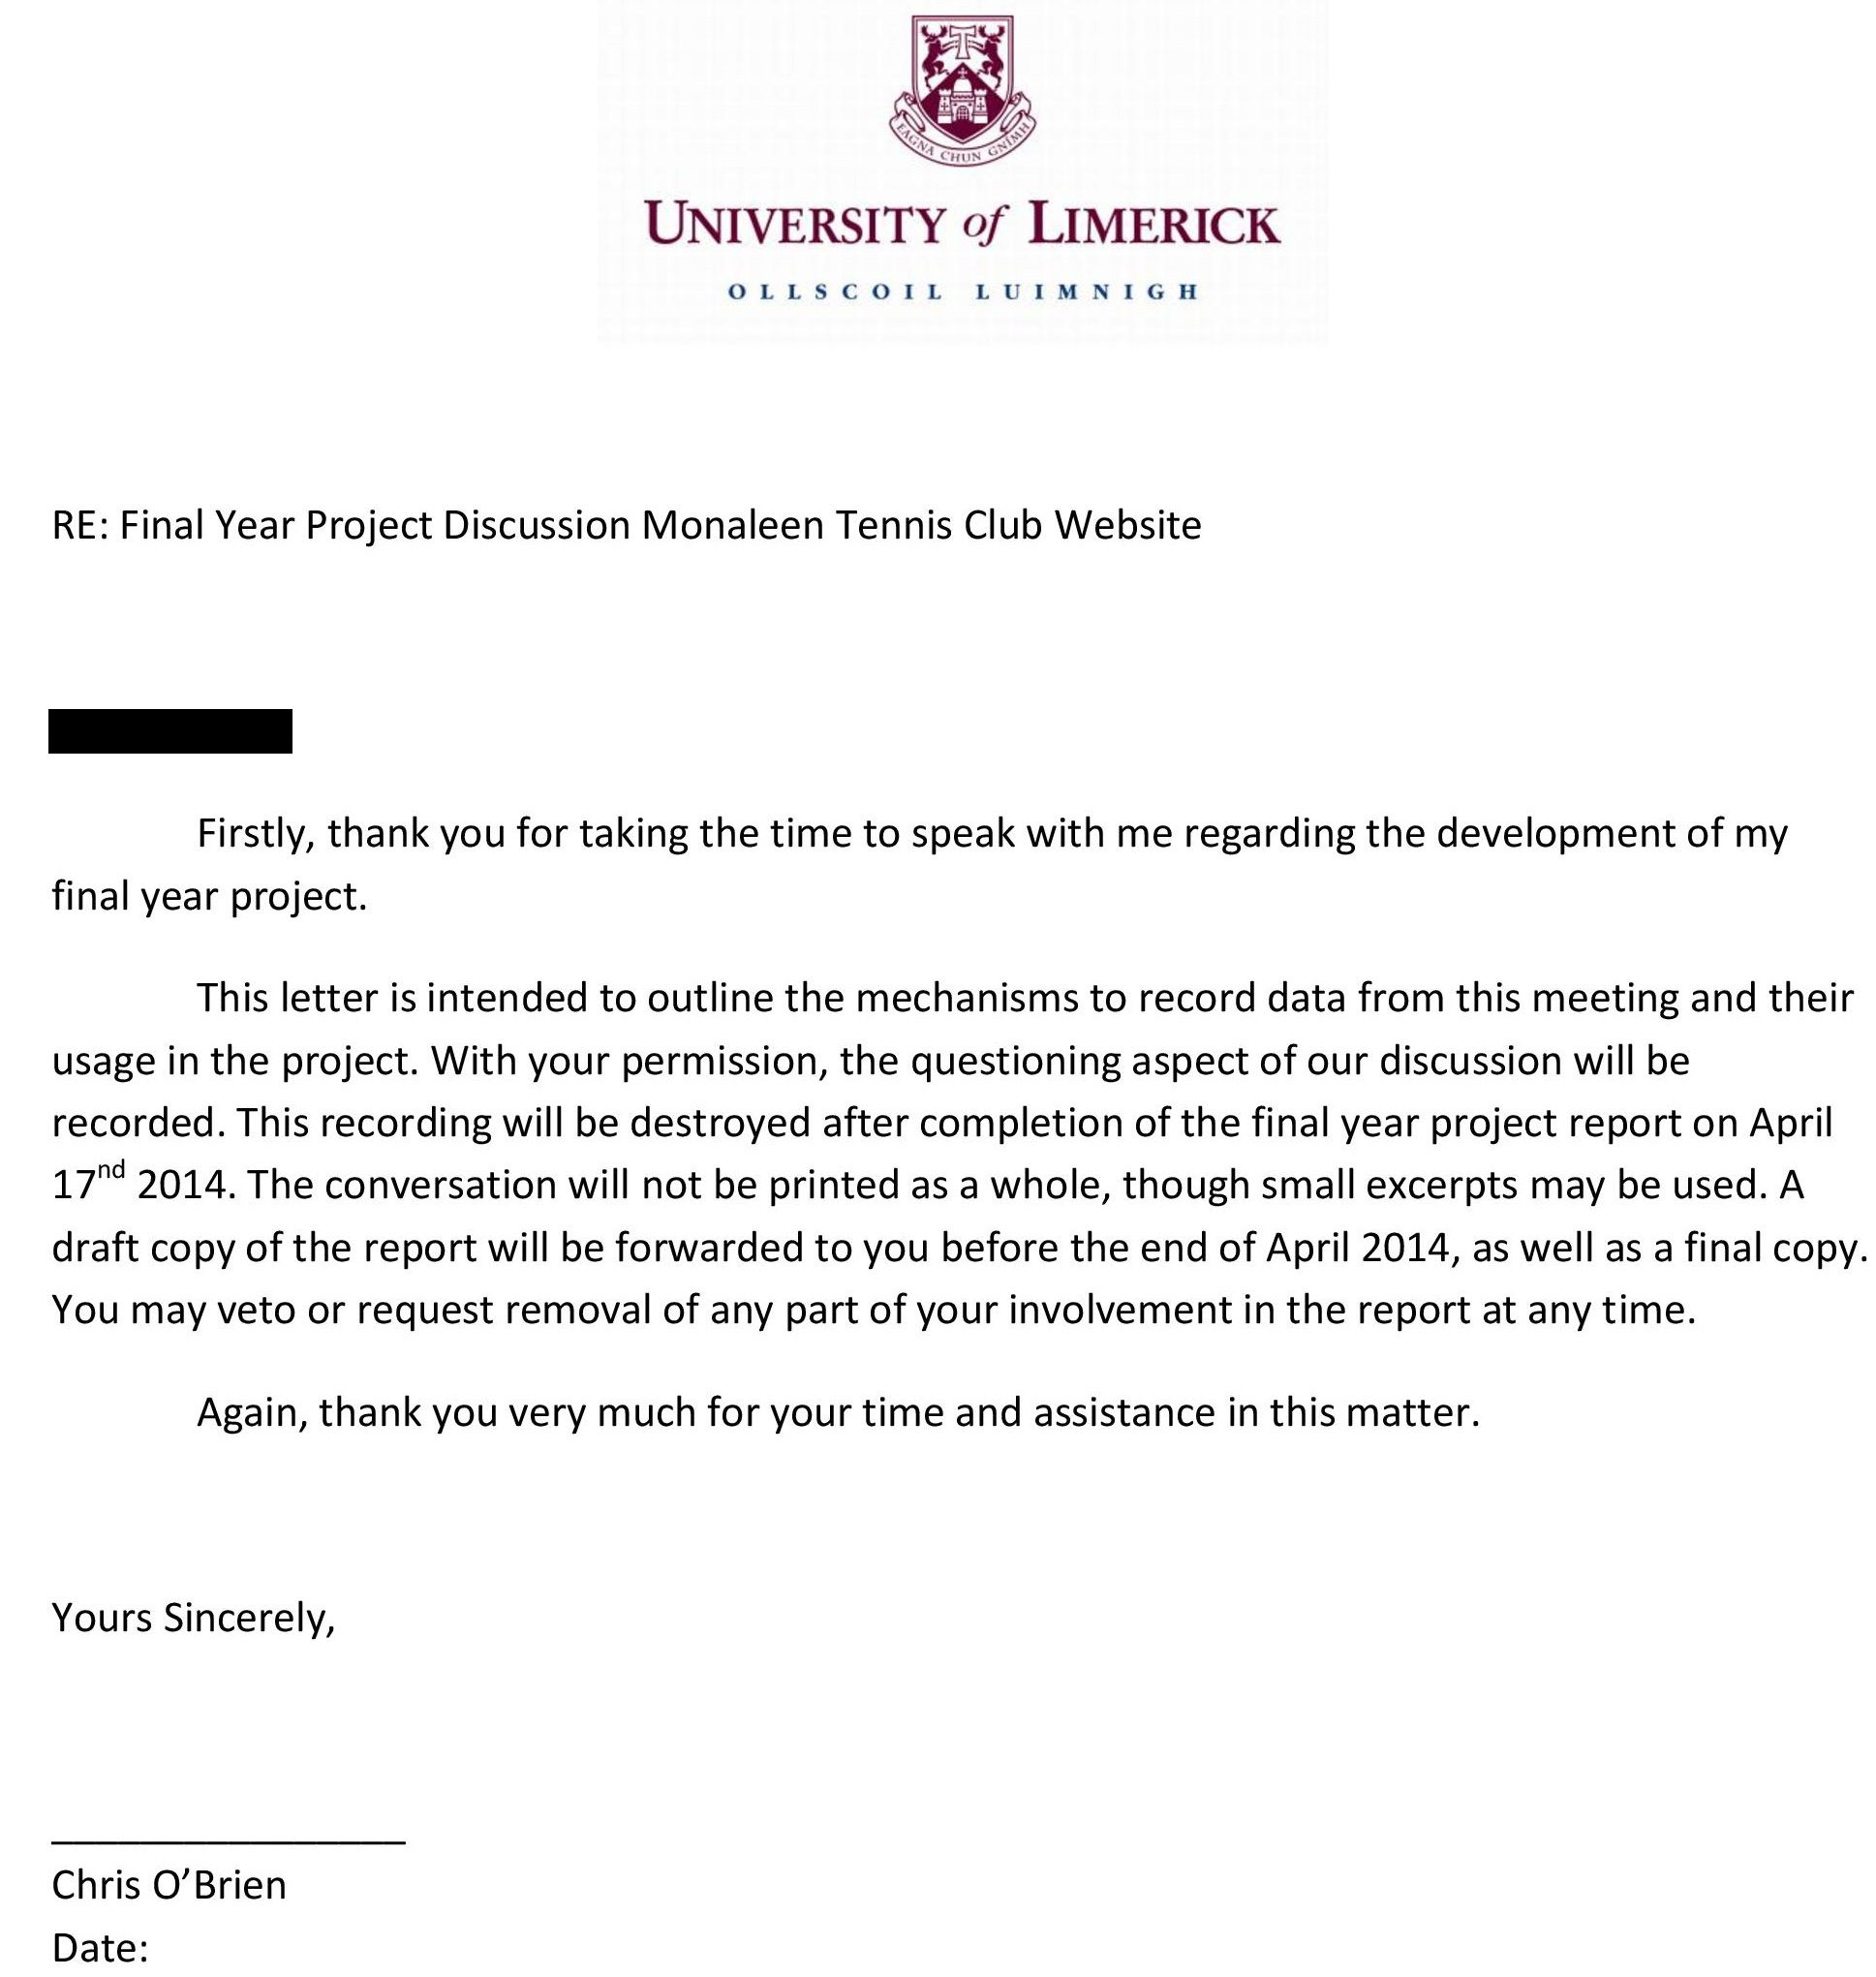
\includegraphics[width=14cm]{letter.jpg}
\end{center}
\caption{Permission letter for interviews}
\label{fig:letter}
\end{figure}
